\documentclass{article}
\usepackage{amsmath}
\usepackage{amssymb}
\usepackage{hyperref}
\usepackage{graphicx}

\begin{document}

\section*{Woche 1}
\subsection*{Aufgabe 1}
\begin{itemize}
    \item Reibung: PVC Rohr mit Stoff
    \item Elektrische Kraft: Kondensation
    \item Influenz: Induzierter Dipol
\end{itemize}
\subsection*{Aufgabe 2}
\begin{center}
    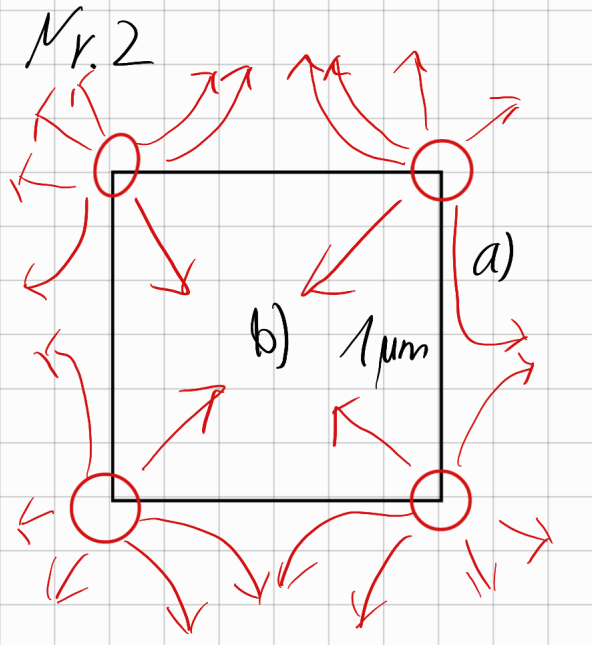
\includegraphics{Abbildungen/Abb.1.png}
\end{center}
\begin{itemize}
    \item[c)] Abstand der Protonen würde gleich bleiben, das ganze System bewegt sich mit.
\end{itemize}
\begin{equation*}
    \vec{F} = \frac{1}{4\pi \varepsilon_0}\cdot\frac{a_1a_2}{r^2}
\end{equation*}
\begin{equation*}
    \varepsilon_0 = 8,85 \cdot 10^{-12} \mathrm{\frac{As}{Vm}}
\end{equation*}
\begin{equation*}
    \vec{F}=\frac{e^2}{4\pi\epsilon r^2}=2,3\cdot 10^{-28} \text{ N}
\end{equation*}
\begin{equation*}
    \text{3 Proton} \rightarrow 2\vec{F}+\frac{1}{2}\vec{F}=5,75 \cdot 10^{-28} \text{ N}
\end{equation*}

\subsection*{Aufgabe 3}
\begin{center}
    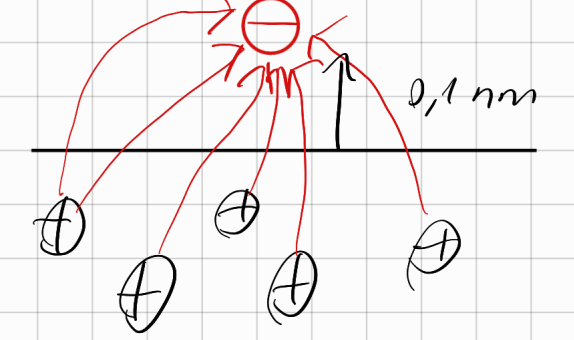
\includegraphics{Abbildungen/Abb.2.png}
\end{center}
\begin{equation*}
    \sigma (r) = \frac{QR}{2\pi (r^2+R^2)^{\frac{3}{2}}}
\end{equation*}
\begin{equation*}
    Q = e, \, R=0,1 \text{ nm}
\end{equation*}
\begin{equation*}
    r = \infty \rightarrow \text{ Plattenlänge}
\end{equation*}
\begin{equation*}
    \sigma (r) = \frac{e \cdot 10^{-10} \text{ m}}{1\pi (\infty \text{ m} +(10^{-10}\text{ m})^2)^{\frac{3}{2}}} = 0
\end{equation*}
\end{document}